\documentclass[solutionorbox,answers]{exam}
% \documentclass[solutionorbox]{exam}

%%%%%%%%%%%%%%%%%%%%%%%%%%%%%%%%%%%%%%%%%%%%%%%%%%%%%%%%%%%%%%%
% Update to change header
\newcommand{\courseName}{CS 577}
\newcommand{\assignmentName}{Assignment 1 -- Discrete Review, Asymptotic Analysis \& Graphs}
\newcommand{\semester}{Summer 2023}
%%%%%%%%%%%%%%%%%%%%%%%%%%%%%%%%%%%%%%%%%%%%%%%%%%%%%%%%%%%%%%%

\usepackage[utf8]{inputenc}
\usepackage[T1]{fontenc}

\usepackage{amsmath}
\usepackage{amsfonts}
\usepackage{amsthm}
\usepackage{booktabs}
\usepackage{tkz-graph}
\usepackage[ruled]{algorithm2e}
\usepackage{graphicx}
\usepackage{multicol}

\usepackage{listings}
\lstset{basicstyle=\ttfamily,
  showstringspaces=false,
  commentstyle=\color{red},
  keywordstyle=\color{blue}
}

\usepackage{hyperref}

\pagestyle{headandfoot}
\runningheadrule
\firstpageheader{\courseName}{\huge \assignmentName}{\semester}
\runningheader{\courseName}
{\assignmentName}
{\semester}
\firstpagefooter{}{}{}
\runningfooter{}{Page \thepage\ of \numpages}{}

\begin{document}

\begin{center}
\fbox{\parbox{5.5in}{\centering
Answer the questions in the boxes provided on the
question sheets. If you run out of room for an answer,
add a page to the end of the document. \\
\vspace{0.1in}
Related Readings: \url{http://pages.cs.wisc.edu/~hasti/cs240/readings/}
}}
\end{center}
\vspace{0.1in}
\makebox[0.48\textwidth]{Name: \underline{Yuhan Wang}} \qquad
\makebox[0.48\textwidth]{Wisc id: \underline{ywang2558} }

\begin{questions}

\section*{Logic}

  \question
  Using a truth table, show the equivalence of the following statements.
\begin{parts}
  \part
  $P \vee (\neg P \wedge Q) \equiv P \vee Q$
  \nopagebreak
  \begin{solutionbox}{2in} \vspace{1em} \\
    \begin{tabular}{c|c|c|c|c|c}
      $P$ & $Q$ & $\neg P$ & $\neg P \wedge Q$ & $P \vee (\neg P \wedge Q)$ & $P \vee Q$ \\
      \hline
      T   & T   & F        & F                 & T                         & T         \\
      T   & F   & F        & F                 & T                         & T         \\
      F   & T   & T        & T                 & T                         & T         \\
      F   & F   & T        & F                 & F                         & F         \\
    \end{tabular}
  \end{solutionbox}
  
  \part
  $\neg P \vee \neg Q \equiv \neg (P \wedge Q)$
  \nopagebreak
  \begin{solutionbox}{2in} \vspace{1em}                                                           \\
    \begin{tabular}{c|c|c|c|c|c}
      $P$ & $Q$ & $\neg P$ & $\neg Q$ & $\neg P \vee \neg Q$ & $\neg (P \wedge Q)$ \\
      \hline
      T   & T   & F        & F        & F                    & F                   \\
      T   & F   & F        & T        & T                    & T                   \\
      F   & T   & T        & F        & T                    & T                   \\
      F   & F   & T        & T        & T                    & T                   \\
    \end{tabular}
  \end{solutionbox}
  
  \part
  $\neg P \vee P \equiv \text{true}$
  \nopagebreak
  \begin{solutionbox}{2in} \vspace{1em} \\
    \begin{tabular}{c|c|c|c}
      $P$ & $\neg P$ & $\neg P \vee P$ & $\text{true}$ \\
      \hline
      T   & F        & T               & T             \\
      F   & T        & T               & T             \\
    \end{tabular}
  \end{solutionbox}
  
  \part
  $P \vee (Q \wedge R) \equiv (P \vee Q) \wedge (P \vee R)$
  \nopagebreak
  \begin{solutionbox}{3in} \vspace{1em} \\
    \begin{tabular}{c|c|c|c|c|c|c|c}
      $P$ & $Q$ & $R$ & $Q \wedge R$ & $P \vee (Q \wedge R)$ & $P \vee Q$ & $P \vee R$ & $(P \vee Q) \wedge (P \vee R)$ \\
      \hline
      T   & T   & T   & T            & T                     & T          & T          & T                              \\
      T   & T   & F   & F            & T                     & T          & T          & T                              \\
      T   & F   & T   & F            & T                     & T          & T          & T                              \\
      T   & F   & F   & F            & T                     & T          & T          & T                              \\
      F   & T   & T   & T            & T                     & T          & T          & T                              \\
      F   & T   & F   & F            & F                     & T          & F          & F                              \\
      F   & F   & T   & F            & F                     & F          & T          & F                              \\
      F   & F   & F   & F            & F                     & F          & F          & F                              \\
    \end{tabular}
  \end{solutionbox}
  
\end{parts}

\newpage
\section*{Sets}


  \question
  Based on the definitions of the sets $A$ and $B$, calculate the following: $|A|$, $|B|$, $A \cup B$, $A \cap B$, $A \setminus B$, $B \setminus A$.

  \begin{parts}
    \part
    $A = \{1, 2, 6, 10\}$ and $B = \{2, 4, 9, 10\}$
    \nopagebreak
    \begin{solutionbox}{2in}
      $|A| = 4$, $|B| = 4$, $A \cup B = \{1, 2, 4, 6, 9, 10\}$, $A \cap B = \{2, 10\}$, $A \setminus B = \{1, 6\}$, $B \setminus A = \{4, 9\}$
    \end{solutionbox}
    \part
    $A = \{x \mid x \in \mathbb{N}\}$ and $B = \{x \in \mathbb{N} \mid x \text{ is even} \}$
    \nopagebreak
    \begin{solutionbox}{2in}
      $|A| = \infty$, $|B| = \infty$, $A \cup B = \{x \mid x \in \mathbb{N}\}$, $A \cap B = \{x \in \mathbb{N} \mid x \text{ is even} \}$, $A \setminus B = \{x \in \mathbb{N} \mid x \text{ is odd} \}$, $B \setminus A = \emptyset$
    \end{solutionbox}

  \end{parts}

\section*{Relations and Functions}

\question
For each of the following relations, indicate if it is reflexive, antireflexive, symmetric, antisymmetric, or transitive.

\begin{parts}
\part
$\{(x,y) : x \le y\}$
\begin{solutionbox}{0.5in}
  It is reflexive, antisymmetric, and transitive.
\end{solutionbox}
\part
$\{(x,y) : x > y\}$
\begin{solutionbox}{0.5in}
  It is antireflexive, antisymmetric, and transitive.
\end{solutionbox}
\newpage
\part
$\{(x,y) : x < y\}$
\begin{solutionbox}{0.5in}
  It is antireflexive, asymmetric, and transitive.
\end{solutionbox}
\part
$\{(x,y) : x = y\}$ 
\begin{solutionbox}{0.5in}
  It is reflexive, symmetric, and transitive.
\end{solutionbox}
\end{parts}

\question
For each of the following functions (assume that they are all $f: \mathbb{Z} \to \mathbb{Z}$), indicate if it is surjective (onto), injective (one-to-one), or bijective.

\begin{parts}
\part
$f(x) = x$
\begin{solutionbox}{0.5in}
  It is bijective.
\end{solutionbox}
\part
$f(x) = 2x - 3$
\begin{solutionbox}{0.5in}
  It is not surjective but it is injective.
\end{solutionbox}
\part
$f(x) = x^2$
\begin{solutionbox}{0.5in}
  It is not surjective and it is not injective.
\end{solutionbox}
\end{parts}
\question
Show that $h(x) = g(f(x))$ is a bijection if $g(x)$ and $f(x)$ are bijections.

\begin{solutionbox}{3in} \\
  \textbf{Injective:} Assume $h(x) = h(y)$. Then $g(f(x)) = g(f(y))$. Since $g(x)$ is injective, $f(x) = f(y)$. Since $f(x)$ is injective, $x = y$. \\
  \textbf{Surjective:} Let $z \in \mathbb{Z}$. Since $g(x)$ is surjective, there exists $y \in \mathbb{Z}$ such that $g(y) = z$. Since $f(x)$ is surjective, there exists $x \in \mathbb{Z}$ such that $f(x) = y$. Then $h(x) = g(f(x)) = g(y) = z$. \\
  Therefore $h(x)$ is bijective.

\end{solutionbox}

\section*{Induction}
\label{sec:induction}

\question
Prove the following by induction.

\begin{parts}
  \part
  $\sum_{i = 1}^n i = n(n+1)/2$
  \begin{solutionbox}{3in}\\
    \textbf{Base case:} $P(1) = 1 = 1(1+1)/2$ \\
    \textbf{Inductive step:} Assume $P(k)$ is true for some $k \ge 1$. Then $\sum_{i = 1}^k i = k(k+1)/2$. \\
    Consider $P(k+1)$. \\
    \begin{align*}
      \sum_{i = 1}^{k+1} i &= \sum_{i = 1}^k i + (k+1) \\
      &= \frac{k(k+1)}{2} + (k+1) \\
      &= \frac{(k+1)(k+2)}{2} \\
    \end{align*}
    Thus $P(k+1)$ is true. \\
    By the principle of mathematical induction, $P(n)$ is true for all $n \ge 1$.
  \end{solutionbox}
  
  \part
  $\sum_{i = 1}^n i^2 = n(n+1)(2n+1)/6$
  \begin{solutionbox}{3in}\\
    $P(1) = 1 = 1(1+1)(2(1)+1)/6$ \\
    Assume $P(k)$ is true for some $k \ge 1$. Then $\sum_{i = 1}^k i^2 = k(k+1)(2k+1)/6$. \\
    Consider $P(k+1)$. \\
    \begin{align*}
      \sum_{i = 1}^{k+1} i^2 &= \sum_{i = 1}^k i^2 + (k+1)^2 \\
      &= \frac{k(k+1)(2k+1)}{6} + (k+1)^2 \\
      &= \frac{(k+1)(k+2)(2k+3)}{6} \\
    \end{align*}
    Thus $P(k+1)$ is true. \\
    By the principle of mathematical induction, $P(n)$ is true for all $n \ge 1$.
  \end{solutionbox}
  
  \part
  $\sum_{i = 1}^n i^3 = n^2(n+1)^2/4$
    \begin{solutionbox}{3.3in}\\
    $P(1) = 1 = 1^2(1+1)^2/4$ \\
    Assume $P(k)$ is true for some $k \ge 1$. Then $\sum_{i = 1}^k i^3 = k^2(k+1)^2/4$. \\
    Consider $P(k+1)$. \\
    \begin{align*}
      \sum_{i = 1}^{k+1} i^3 &= \sum_{i = 1}^k i^3 + (k+1)^3 \\
      &= \frac{k^2(k+1)^2}{4} + (k+1)^3 \\
      &= \frac{(k+1)^2(k^2 + 4k + 4)}{4} \\
      &= \frac{(k+1)^2(k+2)^2}{4} \\
    \end{align*}
    Thus $P(k+1)$ is true. \\
    By the principle of mathematical induction, $P(n)$ is true for all $n \ge 1$.
  \end{solutionbox}
\end{parts}

\section*{Graphs and Trees}
\label{sec:graphs-trees}

\question 
Give the adjacency matrix, adjacency list, edge list, and incidence matrix for the following graph. \\
\begin{minipage}{0.3\linewidth}
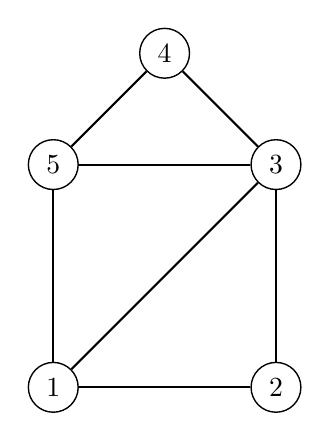
\begin{tikzpicture}
\GraphInit[vstyle=Normal]
\SetGraphUnit{2}
\begin{scope}[rotate=-135]
\Vertices{circle}{1,2,3,5}
\end{scope}
\NOEA[unit=1.414](5){4}
\Edges(1,2,3,5,4,3,1,5)
\end{tikzpicture}
\end{minipage}
\qquad
\begin{minipage}{0.6\linewidth}
\begin{solutionbox}{4in}                                                                          \\
  adjacency matrix:                                                                                   \\
  \begin{tabular}{c|ccccc}
    & 1 & 2 & 3 & 4 & 5 \\
    \hline
    1 & 0 & 1 & 1 & 0 & 1 \\
    2 & 1 & 0 & 1 & 0 & 0 \\
    3 & 1 & 1 & 0 & 1 & 1 \\
    4 & 0 & 0 & 1 & 0 & 1 \\
    5 & 1 & 0 & 1 & 1 & 0 \\
  \end{tabular}                                                                                       \\
  adjacency list:                                                                                     \\
  1: 2, 3, 5                                                                                          \\
  2: 1, 3                                                                                            \\
  3: 1, 2, 4, 5                                                                                       \\
  4: 3, 5                                                                                            \\
  5: 1, 3, 4                                                                                          \\
  edge list:                                                                                          \\
  (1, 2), (1, 3), (1, 5), (2, 3), (3, 4), (3, 5), (4, 5)                                               \\
  incidence matrix: \\
  \begin{tabular}{c|ccccccc}
    & (1,2) & (1,3) & (1,5) & (2,3) & (3,4) & (3,5) & (4,5) \\
    \hline
    1 & 1 & 1 & 1 & 0 & 0 & 0 & 0 \\
    2 & -1 & 0 & 0 & 1 & 0 & 0 & 0 \\
    3 & 0 & -1 & 0 & -1 & 1 & 1 & 0 \\
    4 & 0 & 0 & 0 & 0 & -1 & 0 & 1 \\
    5 & 0 & 0 & -1 & 0 & 0 & -1 & -1 \\
  \end{tabular}   
\end{solutionbox}
\end{minipage}
\question
How many edges are there is a complete graph of size $n$? Prove by induction.

\begin{solutionbox}{3.8in}
  For $n = 1$, there are 0 edges. \\
  Assume $P(k)$ is true for some $k \ge 1$. Then there are $k(k-1)/2$ edges in a complete graph of size $k$. \\
  Consider $P(k+1)$. \\
  \begin{align*}
    \frac{k(k-1)}{2} + k &= \frac{k^2 - k + 2k}{2} \\
    &= \frac{k^2 + k}{2} \\
    &= \frac{k(k+1)}{2} \\
  \end{align*}
  Thus $P(k+1)$ is true. \\
  By the principle of mathematical induction, $P(n)$ is true for all $n \ge 1$.
\end{solutionbox}

\question
Draw all possible (unlabelled) trees with 4 nodes.

\begin{solutionbox}{3.8in}

\end{solutionbox}

\question
Show by induction that, for all trees, $|E| = |V| - 1$.

\begin{solutionbox}{3.8in}
  For $n = 1$, there are 0 edges. \\
  Assume $P(k)$ is true for some $k \ge 1$. Then there are $k-1$ edges in a tree of size $k$. \\
  Consider $P(k+1)$. \\
  \begin{align*}
    k-1 + 1 &= k \\
  \end{align*}
  This is true because a node can only be connected to one other node in a tree. 
  Thus $P(k+1)$ is true. \\
  By the principle of mathematical induction, $P(n)$ is true for all $n \ge 1$.
\end{solutionbox}

\section*{Counting}
\label{sec:counting}

\question
How many 3 digit pin codes are there?

\begin{solutionbox}{0.5in}
  $10^3 = 1000$
\end{solutionbox}

\question
What is the expression for the sum of the $i$th line (indexing starts at 1) of the following: \\
\begin{minipage}{0.1\textwidth}
\begin{align*}
 & 1        \\
 & 2\ 3      \\
 & 4\ 5\ 6    \\
 & 7\ 8\ 9\ 10 \\
 & \vdots
\end{align*}
\end{minipage}
\begin{minipage}{0.89\linewidth}
\begin{solutionbox}{2in} \\
  $i(i+1)/2$ is the last number in the $i$th line. \\
  The first number in the $i$th line is $i(i-1)/2 + 1$. \\
  Thus the sum of the $i$th line is: \\
  \begin{align*}
    (\frac{i(i-1)}{2} + 1 + \frac{i(i+1)}{2}) \times \frac{i}{2} &= \frac{i^3 + i}{2} \\ 
  \end{align*}
\end{solutionbox}
\end{minipage}

\question
A standard deck of 52 cards has 4 suits, and each suit has card number 1 (ace) to 10, a jack, a queen, and a king. A standard poker hand has 5 cards. For the following, how many ways can the described hand be drawn from a standard deck.

\begin{parts}
  \part
  A royal flush: all 5 cards have the same suit and are 10, jack, queen, king, ace.
  \begin{solutionbox}{0.5in}
    4
  \end{solutionbox}

  \part
  A straight flush: all 5 cards have the same suit and are in sequence, but not a royal flush.
  \begin{solutionbox}{0.8in}
    $4 \times 10 - 4 = 36$
  \end{solutionbox}
  
  \part
  A flush: all 5 cards have the same suit, but not a royal or straight flush.
  \begin{solutionbox}{0.8in}
    $4 \times {13 \choose 5} - 4 - 36 = 5108$
  \end{solutionbox}

  \part
  Only one pair (2 of the 5 cards have the same number/rank, while the remaining 3 cards all have different numbers/ranks):
  \begin{solutionbox}{0.8in}
    $13 \times {4 \choose 2} \times {12 \choose 3} \times 4^3 = 1098240$
  \end{solutionbox}
  
\end{parts}

\section*{Proofs}
\label{sec:proofs}

\question
Show that $2x$ is even for all $x \in \mathbb{N}$.

\begin{parts}
  \part
  By direct proof.
  \begin{solutionbox}{2in}
    Let $x \in \mathbb{N}$. \\
    Then $2x / 2 = x \in \mathbb{N}$. \\
    Thus $2x$ is even.
  \end{solutionbox}
  
  \part
  By contradiction.
    \begin{solutionbox}{2in}
    Assume $2x$ is odd. \\
    Then $2x = 2k + 1$ for some $k \in \mathbb{N}$. \\
    But $2x / 2 = x = k + 1/2 \notin \mathbb{N}$. \\
    Thus $2x$ is even.
    \end{solutionbox}
  \end{parts}

\question
For all $x,y \in \mathbb{R}$, show that $|x + y| \le |x| + |y|$. (Hint: use proof by cases.)
\begin{solutionbox}{3in}
  Let $x,y \in \mathbb{R}$. \\
  Note that $|x| \ge x$ and $|x| \ge -x$, and similarly for $y$. \\
  Consider the following cases: \\
  \begin{itemize}
    \item $x + y \ge 0$ \\
      Then $|x + y| = x + y \le |x| + |y|$. 
    \item $x + y < 0$ \\
      Then $|x + y| = -(x + y) = -x - y \le |x| + |y|$.
  \end{itemize}
  Thus $|x + y| \le |x| + |y|$.
\end{solutionbox}

\section*{Program Correctness (and Invariants)}
\label{sec:program-correctness}

\question
For the following algorithms, describe the loop invariant(s) and prove that they are sound and complete.
\begin{parts}
  \part 
  \begin{algorithm}[H]
    \DontPrintSemicolon
    \KwIn{$a$: A non-empty array of integers (indexed starting at 1)}
    \KwOut{The smallest element in the array}
    \Begin{
      $min \gets \infty$\;
      \For{$i \gets 1$ \KwTo len($a$)}{
        \If{$a[i] < min$} {
          $min \gets a[i]$\; 
        }
      }
      \Return{$min$}\;
    }
    \caption{findMin}
  \end{algorithm}
  \begin{solutionbox}{5.9in}
    For the loop invariant, we use the following: \\ 
    \begin{itemize}
      \item \textbf{Initialization}: \\
        Before the first iteration, $min = \infty$. \\
        Thus $min$ is the smallest element in the array.
      \item \textbf{Maintenance}: \\
        Assume $min$ is the smallest element in the array before the $i$th iteration. \\
        Then $min \le a[i]$. \\
        After the $i$th iteration, $min$ is updated to $a[i]$ if $a[i] < min$. \\
        Thus $min$ is the smallest element in the array after the $i$th iteration.
      \item \textbf{Termination}: \\
        The loop terminates when $i = $ len($a$) + 1. \\
        By the maintenance property, $min$ is the smallest element in the array. \\
        Thus $min$ is the smallest element in the array.
    \end{itemize}
    For soundness, we have shown that the loop invariant holds before the first iteration, and that if it holds before an iteration, it holds after the iteration. \\
    For completeness, we have shown that if the loop terminates, the loop invariant holds for all inputs $a$.
  \end{solutionbox}

    \part 
  \begin{algorithm}[H]
    \DontPrintSemicolon
    \KwIn{$a$: A non-empty array of integers (indexed starting at 1)}
    \KwOut{$a$ sorted from largest to smallest}
    \SetKw{Break}{break}
    \Begin{
      \For{$i \gets 2$ \KwTo len($a$)}{
        $val \gets a[i]$\;
        \For{$j \gets 1$ \KwTo $i - 1$}{
          \If{$val > a[j]$} {
            shift $a[j..i-1]$ to $a[j+1..i]$\;
            $a[j] \gets val$\;
            \Break
          }
        }
      }
      \Return{$a$}\;
    }
    \caption{InsertionSort}
  \end{algorithm}
  \begin{solutionbox}{5.9in}
    \begin{itemize}
      \item \textbf{Sound}: \\
        The loop invariant is that $a[1..i-1]$ is sorted from largest to smallest. \\
        This is true before the first iteration of the outer loop, since $a[1]$ is trivially sorted. \\
        Now assume that $a[1..i-2]$ is sorted from largest to smallest. \\
        Then the inner loop shifts $a[j..i-1]$ to $a[j+1..i]$ until $a[j] \ge val$. \\
        Thus $a[1..i-1]$ is sorted from largest to smallest. \\

      \item \textbf{Complete}: \\
        The loop terminates when $j = 1$ and $a[j] \ge val$. \\
        Thus $a[1..i]$ is sorted from largest to smallest. \\
        Since $i$ is incremented after each iteration of the outer loop, the algorithm terminates with $a[1..len(a)]$ sorted from largest to smallest for all inputs $a$.
    \end{itemize}
  \end{solutionbox}
  
\end{parts}
\section*{Recurrences}
\label{sec:recurrences}

\question
Solve the following recurrences.

\begin{parts}
  \part
  $c_0 = 1; c_{n} = c_{n-1} + 4$

  \begin{solutionbox}{3.7in}
    $c_n = c_{n-1} + 4 = c_{n-2} + 4 + 4 = c_{n-3} + 4 + 4 + 4 = \ldots = c_0 + 4n = 1 + 4n$
  \end{solutionbox}

  \part
  $d_0 = 4; d_{n} = 3 \cdot d_{n-1} $

  \begin{solutionbox}{3.7in}
    $d_n = 3 \cdot d_{n-1} = 3 \cdot 3 \cdot d_{n-2} = 3^2 \cdot 3 \cdot d_{n-3} = \ldots = 3^n \cdot 4$
  \end{solutionbox}

  \part
  $T(1) = 1; T(n) = 2T(n/2) + n$ (An upper bound is sufficient.)

  \begin{solutionbox}{3.9in} \\
    $T(n) = 2T(n/2) + n = 2(2T(n/4) + n/2) + n = 2^2T(n/2^2) + 2n = \ldots = 2^kT(n/2^k) + kn$ \\
    $n/2^k = 1 \implies k = \log_2 n$ \\
    $T(n) = 2^{\log_2 n}T(1) + n\log_2 n = n + n\log_2 n = O(n\log n)$
  \end{solutionbox}

  \part
  $f(1) = 1; f(n) = \sum_{1}^{n-1}\left(i \cdot f(i)\right)$\\ (Hint: compute $f(n+1)-f(n)$ for $n>1$)

  \begin{solutionbox}{3.9in} \\
    $f(2) = \sum_{1}^{1}\left(i \cdot f(i)\right) = 1 \cdot f(1) = 1$ \\
    $f(n+1) - f(n) = \sum_{1}^{n}\left(i \cdot f(i)\right) - \sum_{1}^{n-1}\left(i \cdot f(i)\right) = n \cdot f(n)$ \\
    $f(n+1) - f(n) = n \cdot f(n) $ \\
    $f(n+1) = (n+1) \cdot f(n) $ \\
    $f(n+1) = (n+1) \cdot n \cdot f(n-1) = (n+1) \cdot n \cdot (n-1) \cdot f(n-2) = \ldots = (n+1)! / 2$ \\
    $f(n) = n! / 2$
  \end{solutionbox}
\end{parts}

\section*{Coding Question: Hello World}

Most assignments will have a coding question. You can code in C, C++, C\#, Java, Python, or Rust. You will submit a Makefile and a source code file.
\vspace{-0.5cm}

\paragraph{Makefile:} In the Makefile, there needs to be a build command and a run command. Below is a sample Makefile for a C++ program. You will find this Makefile in assignment details. Download the sample Makefile and edit it for your chosen programming language and code.

\lstinputlisting[language=Make]{Makefile}

\newpage
\question{\bf{HelloWorld Program Details}}
%\paragraph

The input will start with a positive integer, giving the number of instances that follow. For each instance, there will be a string. For each string $s$, the program should output Hello, $s$! on its own line.

A sample input is the following:
\begin{verbatim}
3
World
Marc
Owen
\end{verbatim}

The output for the sample input should be the following:
\begin{verbatim}
Hello, World!
Hello, Marc!
Hello, Owen!
\end{verbatim}

\section*{Asymptotic Analysis}

  \question \textit{Kleinberg, Jon. Algorithm Design (p. 67, q. 3, 4).} Take the following list of functions and arrange them in ascending order of growth rate. That is, if function $g(n)$ immediately follows function $f(n)$ in your list, then it should be the case that $f(n)$ is $O(g(n))$. 

\begin{parts}
  \part
  $f_1(n) = n^{2.5}$ \\
  $f_2(n) = \sqrt{2n}$ \\
  $f_3(n) = n + 10$ \\
  $f_4(n) = 10n$ \\
  $f_5(n) = 100n$ \\
  $f_6(n) = n^2 \log{n}$
  \begin{solutionbox}{1in} \vspace{1em} \\
    $f_2(n), f_3(n), f_4(n), f_5(n), f_6(n), f_1(n)$
  \end{solutionbox}
  
  \part
  $g_1(n) = 2^{\log{n}}$ \\
  $g_2(n) = 2^n$ \\
  $g_3(n) = n(\log{n})$ \\
  $g_4(n) = n^{4/3}$ \\
  $g_5(n) = n^{\log{n}}$ \\
  $g_6(n) = 2^{(2^n)}$ \\
  $g_7(n) = 2^{(n^2)}$
  \nopagebreak
  \begin{solutionbox}{1in} \vspace{1em} \\
    $g_1(n), g_3(n), g_4(n), g_5(n), g_2(n), g_7(n), g_6(n)$
  \end{solutionbox}
  
\end{parts}

\pagebreak

  \question \textit{Kleinberg, Jon. Algorithm Design (p. 68, q. 5).} Assume you have a positive, non-decreasing function $f$ and a positive, non-decreasing function $g$ such that $g(n) \geq 2$ and $f(n)$ is $O(g(n))$. For each of the following statements, decide whether you think it is true or false and give a proof or counterexample.

\begin{parts}
  \part
  $\log_2{f(n)}$ is $O(\log_2{g(n)})$ 

  \begin{solutionbox}{2.5in} \vspace{1em} \\
    True. \\
    $f(n)$ is $O(g(n))$ \\
    $f(n) \leq c \cdot g(n)$ \\
    $\log_2{f(n)} \leq \log_2{c \cdot g(n)}$ \\
    $\log_2{f(n)} \leq \log_2{c} + \log_2{g(n)}$ \\
    $\log_2{f(n)}$ is $O(\log_2{g(n)})$ \\
  \end{solutionbox}
  
    \part 
    $2^{f(n)}$ is $O(2^{g(n)})$
    
    \nopagebreak
    \begin{solutionbox}{2in} \vspace{1em}                                                           \\
      True. \\
      $f(n)$ is $O(g(n))$ \\
      $f(n) \leq c \cdot g(n)$ \\
      $2^{f(n)} \leq 2^{c \cdot g(n)}$ \\
      $2^{f(n)} \leq 2^{c} \cdot 2^{g(n)}$ \\
      $2^{f(n)}$ is $O(2^{g(n)})$ \\
    \end{solutionbox}

\part
    $f(n)^2$ is $O(g(n)^2)$
    
    \nopagebreak
    \begin{solutionbox}{2in} \vspace{1em} \\
      True. \\
      $f(n)$ is $O(g(n))$ \\
      $f(n) \leq c \cdot g(n)$ , $f(n) \geq 0$ , $g(n) \geq 0$ \\
      $f(n)^2 \leq c^2 \cdot g(n)^2$ \\
      $f(n)^2$ is $O(g(n)^2)$ \\
  \end{solutionbox}
  
\end{parts}

\pagebreak

\question \textit{Kleinberg, Jon. Algorithm Design (p. 68, q. 6).} You're given an array $A$ consisting of $n$ integers. You'd like to output a two-dimensional $n$-by-$n$ array $B$ in which $B[i, j]$ (for $i < j$) contains the sum of array entries $A[i]$ through $A[j]$ — that is, the sum $A[i]+ A[i + 1]+... + A[j]$. (Whenever $i \geq j$, it doesn't matter what is output for $B[i,j]$.)  
Here's a simple algorithm to solve this problem. 

\begin{lstlisting}
for i = 1 to n
  for j = i + 1 to n  
    add up array entries A[i] through A[j]
    store the result in B[i, j]
  endfor  
endfor 
\end{lstlisting}

\begin{parts}

\part For some function $f$ that you should choose, give a bound of the form $O(f(n))$ on the running time of this algorithm on an input of size $n$ (i.e., a bound on the number of operations performed by the algorithm).

\begin{solutionbox}{0.65in}    \vspace{1em}     
  For each $i$, the inner loop runs $n-i$ times. \\
  $T(n) = \sum_{i=1}^{n} (n-i) = \sum_{i=1}^{n} n - \sum_{i=1}^{n} i = n^2 - \frac{n(n+1)}{2} = \frac{n(n-1)}{2} = O(n^2)$ \\
\end{solutionbox}

\part For this same function $f$, show that the running time of the algorithm on an input of size $n$ is also $\Omega(f(n))$. (This shows an asympto tically tight bound of $\Theta(f(n))$ on the running time.)

\begin{solutionbox}{1.25in}    \vspace{1em}     \\
  For each $i$, the inner loop runs $n-i$ times. \\
  $T(n) = \sum_{i=1}^{n} (n-i) = \sum_{i=1}^{n} n - \sum_{i=1}^{n} i = n^2 - \frac{n(n+1)}{2} = \frac{n(n-1)}{2} = \Omega(n^2)$ \\
\end{solutionbox}

\part Although the algorithm provided is the most natural way to solve the problem, it contains some highly unnecessary sources of inefficiency. Give a different algorithm to solve this problem, with an asymptotically better running time. In other words, you should design an algorithm with running time $O(g(n))$, where $\lim_{n \to \infty}{\frac{g(n)}{f(n)}} = 0$. 

\begin{solutionbox}{2.95in}    \vspace{1em}     \\
  Let $S$ be an array of size $n$ where $S[i] = \sum_{j=1}^{i} A[j]$ \\
  $S[1] = A[1]$ \\
  $S[i] = S[i-1] + A[i]$ \\
  $B[i,j] = S[j] - S[i-1]$ \\
  $T(n) = n + 1 = O(n)$ \\
  This algorithm is $O(n)$ and satisfies the requirements. \\
\end{solutionbox}

\end{parts}


\pagebreak
\section*{Graphs}

\question Given the following graph, list a possible order of traversal of nodes by breadth-first search and by depth-first search. Consider node 1 to be the starting node.

\begin{minipage}{0.3\linewidth}
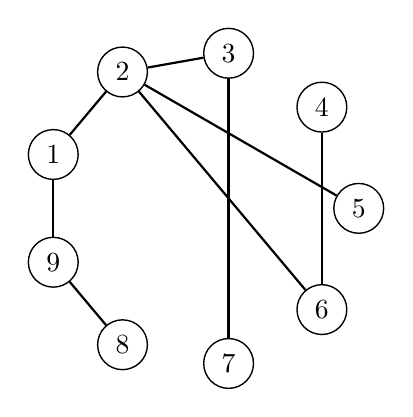
\begin{tikzpicture}
\GraphInit[vstyle=Normal]
\SetGraphUnit{2}
\Vertices{circle}{5,4,3,2,1,9,8,7,6}
\Edges(8,9,1,2,5)
\Edges(2,3,7)
\Edges(4,6)
\Edges(2,6)
\end{tikzpicture}
\end{minipage}
\qquad
\begin{minipage}{0.6\linewidth}
\begin{solutionbox}{1.7in}    \vspace{1em}                                                            \\
  Breadth-First Search: in the groups, order doesn't matter

   1, [2, 9], [3, 5, 6, 8] , [4, 7]   \\

  Depth-First Search: not an exhaustive list of solutions \\
  Some possible solutions: \\
   1, 9, 8, 2, 3, 7, 6, 4, 5 \\
   1, 2, 3, 7, 6, 4, 5, 9, 8 \\
   1, 2, 6, 4, 5, 3, 7, 9, 8
\end{solutionbox}
\end{minipage}

\question \textit{Kleinberg, Jon. Algorithm Design (p. 108, q. 5).} A binary tree is a rooted tree in which each node has at most two children. Show by induction that in any binary tree the number of nodes with two children is exactly one less than the number of leaves. 

\nopagebreak

\begin{solutionbox}{5in}    \vspace{1em}    \\                                                        
  \textbf{Base Case:} \\
  A tree with one node has no leaves and no nodes with two children. \\
  \textbf{Inductive Hypothesis:} \\
  Assume that for a tree with $n$ nodes, the number of nodes with two children is exactly one less than the number of leaves. \\
  \textbf{Inductive Step:} \\
  Consider a tree with $n+1$ nodes. Let us add a node to the tree with $n$ nodes. \\
  If we add to a leaf, then the number of leaves and nodes with two children both stay the same. \\
  If we add to a node with one child, then the number of leaves and nodes with two children both increase by one. \\
  Thus the number of nodes with two children is still one less than the number of leaves. \\
\end{solutionbox}
\pagebreak
\question \textit{Kleinberg, Jon. Algorithm Design (p. 108, q. 7).} Some friends of yours work on wireless networks, and they're currently studying the properties of a network of $n$ mobile devices. As the devices move around, they define a graph at any point in time as follows: 

{\leftskip=1cm\relax
 \rightskip=1cm\relax
 There is a node representing each of the $n$ devices, and there is an edge between device $i$ and device $j$ if the physical locations of $i$ and $j$ are no more than 500 meters apart. (If so, we say that $i$ and $j$ are “in range” of each other.)
 \par}

They'd like it to be the case that the network of devices is connected at all times, and so they've constrained the motion of the devices to satisfy the following property: at all times, each device $i$ is within 500 meters of at least $\frac{n}{2}$ of the other devices. (We'll assume $n$ is an even number.) What they'd like to know is: Does this property by itself guarantee that the network will remain connected? \\

Here’s a concrete way to formulate the question as a claim about graphs.\\

\textbf{Claim: Let $G$ be a graph on $n$ nodes, where $n$ is an even number. If every node of $G$ has degree at least $\frac{n}{2}$, then $G$ is connected.} \\

Decide whether you think the claim is true or false, and give a proof of either the claim or its negation. 

\begin{solutionbox}{4.5in} \vspace{1em}    \\
  \textbf{Claim: Let $G$ be a graph on $n$ nodes, where $n$ is an even number. If every node of $G$ has degree at least $\frac{n}{2}$, then $G$ is connected.} \\
  \textbf{Proof:} \\
  Assume that $G$ is not connected. \\
  Then there exists a node $v$ such that there is no path from $v$ to some other node $u$. \\
  Since $G$ is not connected, there must be at least one other node $w$ such that there is no path from $w$ to $u$. \\
  
  \end{solutionbox}

\pagebreak



\section*{Coding Question: DFS}
\question
Implement depth-first search in either C, C++, C\#, Java, Python, or Rust. Given an undirected graph with $n$ nodes and $m$ edges, your code should run in $O(n + m)$ time. Remember to submit a makefile along with your code, just as with the first coding question.\\

\textbf{Input:} the first line contains an integer $t$, indicating the number of instances that follows. For each instance, the first line contains an integer $n$, indicating the number of nodes in the graph. Each of the following $n$ lines contains several space-separated strings, where the first string $s$ represents the name of a node, and the following strings represent the names of nodes that are adjacent to node $s$.

The input order of the nodes is important as it will be used as the tie-breaker. For example, consider two consecutive lines of an instance:
\begin{verbatim}
0, F
B, C, a
\end{verbatim}
Note that the tie break priority would be 0 $<$ F $<$ B $<$ C $<$ a.\\

\textbf{Input constraints:}
\begin{itemize}
    \item $1 \leq t \leq 1000$
    \item $1 \leq n \leq 100$
    \item Strings only contain alphanumeric characters
    \item Strings are guaranteed to be the names of the nodes in the graph.
\end{itemize}

\textbf{Output:} for each instance, print the names of nodes visited in depth-first traversal of the graph, \emph{with ties between nodes visiting the first node in input order}. Start your traversal with the first node in input order. The names of nodes should be space-separated, and each line should be terminated by a newline.\\

\textbf{Sample:}
\begin{multicols}{2}
\textbf{Input:} 
\begin{verbatim}
2
3
A B
B A
C
9
1 2 9
2 1 6 5 3
4 6
6 2 4
5 2
3 2 7
7 3
8 9
9 1 8
\end{verbatim}
\columnbreak
\textbf{Output:} 
\begin{verbatim}
A B C
1 2 6 4 5 3 7 9 8
\end{verbatim}
\end{multicols}

The sample input has two instances. 
The first instance corresponds to the graph below on the left. 
The second instance corresponds to the graph below on the right.
\begin{center}
\begin{minipage}{0.3\linewidth}
    \begin{tikzpicture}
        \GraphInit[vstyle=Normal]
        \SetGraphUnit{2}
        \Vertices{circle}{A,B,C}
        \Edges(A,B)
    \end{tikzpicture}
\end{minipage}
\qquad\qquad
\begin{minipage}{0.3\linewidth}
    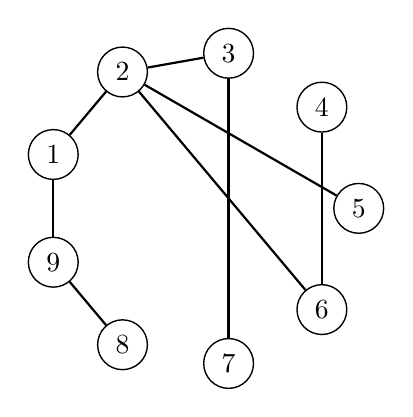
\begin{tikzpicture}
        \GraphInit[vstyle=Normal]
        \SetGraphUnit{2}
        \Vertices{circle}{5,4,3,2,1,9,8,7,6}
        \Edges(8,9,1,2,5)
        \Edges(2,3,7)
        \Edges(4,6)
        \Edges(2,6)
    \end{tikzpicture}
\end{minipage}

\hfill
\end{center}

\end{questions}

\end{document}
